\chapter{Distribuição Gaussiana}
\label{sec:gauss}

\vspace{-0.7cm}

\section*{Valor médio, Desvio Padrão e Densidade de Probabilidade}

Sejam $N$ medições aleatórias independentes de uma grandeza qualquer, $x_1, x_2, x_3, ... , x_N$. Como alguns dos valores $x_i$ medidos podem ser repetidos, podemos dizer que para esta grandeza temos $M$ {\bf eventos} possíveis de medida tal que $M \leq N$ e eles são: $y_1, y_2, ..., y_M$. Então, podemos definir a {\bf frequência de ocorrência} do evento $y_i$ como $N(y_i)$ de forma tal que:
\begin{equation}
\sum_{i=1}^M N(y_i) = N.
\end{equation}
\noindent

Desta forma, podemos definir a {\bf frequência relativa} como a fração de eventos $y_i$ em relação ao número total de eventos $N$, dada por:
\begin{equation}
F(y_i) = \frac{N(y_i)}{N},
\label{eq:freqrel}
\end{equation}
\noindent
de forma que (mostrar):
\begin{equation}
\sum_{i=1}^M F(y_i) = 1.
\end{equation}
\noindent

Se o processo é repetido indefinidamente, ou seja, $N \longrightarrow \infty$, a frequência relativa é interpretada como a {\bf probabilidade de ocorrência} do evento $y_i$:
\begin{equation}
P(y_i) = \lim_{N \to \infty} F(y_i) = \lim_{N \to \infty} \frac{N(y_i)}{N},
\end{equation}
\noindent
e como sabemos que $0  \leq N(y_i) \leq N$, então $0  \leq P(y_i) \leq 1$.

No Capítulo~\ref{stat} da parte Conceitos Básicos definimos os conceitos de valor médio e desvio padrão. Agora podemos re-escrever estas definições em função da frequência relativa, obtendo:

\begin{enumerate}
\item {\bf Valor médio}
\begin{equation}
\bar{x} = \sum_{i = 1}^M F(x_i){x_i},
\end{equation}
\noindent

\item {\bf Variância $V[x] = \sigma^2$}
\begin{equation}
\sigma^2 = \sum_{i=1}^M (x_i - \bar{x})^2 F(x_i)
\end{equation}
\noindent
\vspace{-1.cm}
\end{enumerate}
 
%Frequentemente ocorre que num processo aleatório o valor médio para a determinação de uma grandeza pode resultar em um número muito grande de valores possíveis. A medida do período de oscilação de um pêndulo simples é um exemplo. 

Quan\-do realizamos observações experimentais utilizamos instrumentos que determinam os valores de grandezas que são continuamente distribuídas. Os resultados são truncados até o limite da precisão de medida do instrumento utilizado. Por exemplo, um cronômetro usual mede intervalos de tempo com precisão de um centésimo de segundo. Isto significa que intervalos de tempo menores que este valor não podem ser medidos com este instrumento. Assim, os resultados obtidos serão representados por um número finito de valores, mesmo que a variável observada seja contínua. Algumas vezes, o número de valores possíveis medidos, mesmo que finito, pode ser muito grande, e para estes casos é conveniente agrupa-los em intervalos.  Desta forma o conjunto de medidas diferentes fica reduzido sem que a informação da amostra original seja perdida.

Consideremos novamente $N$ medições aleatórias independentes de uma grandeza qualquer, $x_1, x_2, x_3, ... , x_N$. Para estes casos, definimos como o mesmo evento todo resultado da realização do processo aleatório $y$ que caia num intervalo de valores $\Delta y$, de forma que o evento agora será caracterizado por $\{y_i, \Delta y\}$: 
\begin{equation}
y_i - \frac{\Delta y}{2} \leq x_j  < y_i + \frac{\Delta y}{2}.
\end{equation}

A probabilidade de ocorrência do evento $\{y_i, \Delta y \}$ é definida por:
\begin{equation}
P(y_i) = \Delta P_i
\end{equation}
\noindent
onde $\Delta P_i$ é a probabilidade de encontrarmos como resultado da realização do processo aleatório, valores no intervalo $\{y_i - \frac{\Delta y}{2}, y_i +	 \frac{\Delta y}{2}\}$. Para intervalos $\Delta y$ pequenos, podemos escrever a seguinte relação:
\begin{equation}
P(y_i) = \Delta P_i = p(y_i) \Delta y
\end{equation}
\noindent
onde $p(y_i)$ é denominada de densidade de probabilidade do evento aleatório $y_i$. E se $\Delta y \longrightarrow 0$, então $\Delta P_i$ e $\Delta y$ são infinitesimais podendo escrever a densidade de probabilidade como:
\begin{equation}
p(y) = \frac{dP}{dy}
\end{equation}
\noindent
sendo que: 
\begin{equation}
\int_{-\infty}^{+\infty} \! p(y) \, \mathrm{d}y = 1
\end{equation}
\noindent

Em $N$ repetições de um processo aleatório real, a aproximação experimental para a probabilidade de realização de um evento é a frequência relativa $F(y_i)$, definida na equação~\ref{eq:freqrel}.  Assim, a densidade de probabilidade experimental $p_{exp}(y_i)$ de ocorrência do evento $\{y_i, \Delta y \}$ é dada por:  
\begin{equation}
p_{exp}(y_i) = \frac{F(y_i)}{\Delta y}.
\end{equation}
\noindent

Para o caso contínuo e utilizando o conceito de densidade de probabilidade, o valor médio ($\mu$) e a variância ($\sigma^2$) podem ser escritos da seguinte forma: 

\begin{enumerate}
\item {\bf Valor médio}
\begin{equation}
\mu = \int_{-\infty}^{+\infty} \! y~p(y) \, \mathrm{d}y. 
\end{equation}
\noindent

\item {\bf Variância $V[y] = \sigma^2$}
\begin{equation}
\sigma^2 =\int_{-\infty}^{+\infty} \! (y-\mu)^2~p(y) \, \mathrm{d}y. 
\end{equation}
\end{enumerate}



\section*{Função de Laplace-Gauss}

Em muitas situações experimentais utilizamos {\bf distribuições Gaussianas} para interpretar nossos resultados físicos, em parte porque os fundamentos teóricos das medições realizadas se correspondem com distribuições Gaussianas ou porque a experiência tem nos mostrado que a estatística de Gauss nos proporciona uma descrição razoavelmente acurada dos vários eventos reais. Na distribuição Gaussiana, a densidade de probabilidade é dada por:
\begin{equation}
p(x) = G(x) = \frac{1}{\sqrt{2 \pi \sigma^2}}~e^{-\frac{1}{2}\left(\frac{x - \mu}{\sigma}\right)^2}
\label{eq:gauss}
\end{equation}
\noindent
onde $\mu $ é o valor médio e $\sigma$ o desvio padrão da distribuição, dados pelas equações discutidas anteriormente.

Na Figura~\ref{fig:gauss} apresentamos a função Gaussiana de densidade de probabilidade para a variável continua $x$.  Esta função é também chamada de função de Laplace-Gauss ou função Normal. O gráfico da função Gaussiana é uma curva simétrica em forma de ``sino'' \-com uma altura máxima dada por $G_{max} = 1/\sqrt{2 \pi \sigma^2}$. Pode ser mostrado a partir da equação~\ref{eq:gauss} que 
$\sigma$ é a meia largura da curva na altura correspondente a $\sim 0,61 G_{max}$ e que a área sob a curva entre $\mu - \sigma$ e $\mu + \sigma$ (região pintada na Figura~\ref{fig:gauss}) corresponde a 68,3\% da área total. Isto quer dizer que a probabilidade de medirmos um valor no intervalo $\mu \pm \sigma$ é 68,3\%. Seguindo o mesmo procedimento, podemos mostrar que a probabilidade de encontrarmos um valor entre  $\mu \pm 2\sigma$ é 95,4\% e entre $\mu \pm 3\sigma$ é 99,7\%.


\begin{figure}[t]
\begin{center}
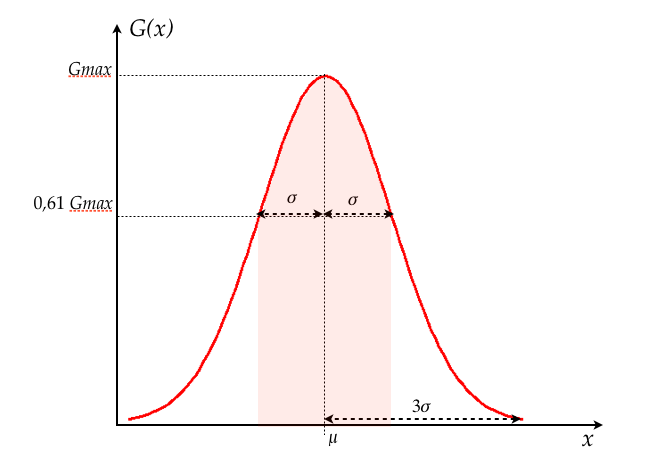
\includegraphics[width=14cm]{fig/Gauss.png}
%\vspace{-0.7cm}
\caption{\label{fig:gauss} Representação da função Gaussiana.}
\end{center}
%\vspace{13cm}
\end{figure}

